\subsection{Validating MLMC Stochastic Heat Implementation}\label{sec:stoch_heat_validation}

We now validate our MLMC implementation for the Stochastic Heat Equation.
We do this by demonstrating that our MLMC estimator converges to the correct, 
analytically-derived expected values for our chosen quantities of interest for
all three coupling strategies, and that the observed 
growth and decay rates align with those derived for squared amplitudes. 
We also discuss the resulting validation charts as they vary for different coupling 
strategies.

We first consider the squared Fourier amplitude. We use the first Fourier mode, 
for which the true value we know to 
be $\approx 0.10$
via \eqref{eq:squared_amplitude_analytic}.
For each of the three coupling strategies (NN, CC, and FE) the following was done. 
A preliminary run with 10,000 samples across each of 
the first six levels was performed to obtain 
empirical estimates of the key MLMC 
parameters ($\alpha, \beta, \gamma$) via linear regression. 
The adaptive MLMC algorithm (Algorithm \ref{alg:mlmc_detailed}) was then 
executed using those estimated rates for a range of 
target RMSEs, $\varepsilon \in \{0.1, 0.05, 0.02, 0.01, 0.005, 0.001\}$. 
This is in line with the methodology outlined in Section
\ref{sec:mlmc_algorithm}.

The results of this analysis are presented in Figure \ref{fig:she_validation_combined}, 
the estimated rates summarised in Table \ref{tab:she_decay_rates}.

\begin{table}[htbp]
    \centering
    \begin{tabular}{|l|c|c|r|}
        \hline
        \textbf{Coupling Method} & \textbf{$\alpha$} & \textbf{$\beta$} & \textbf{$\gamma$} \\
        \hline
        Nearest Neighbour & 2.0 & 2.07 & 3.02\\
        Central Coupling & 1.86 & 2.08 & 3.02 \\
        Finite Element & 1.96 & 4.0 & 3.0 \\
        \hline
    \end{tabular}
    \caption{Empirically estimated rates for the Squared Amplitude QoI.}
    \label{tab:she_decay_rates}
\end{table}

\begin{figure}[htbp]
    \centering
    \begin{subfigure}{\textwidth}
        \centering
                \begin{subfigure}[b]{0.48\textwidth}
            \centering
            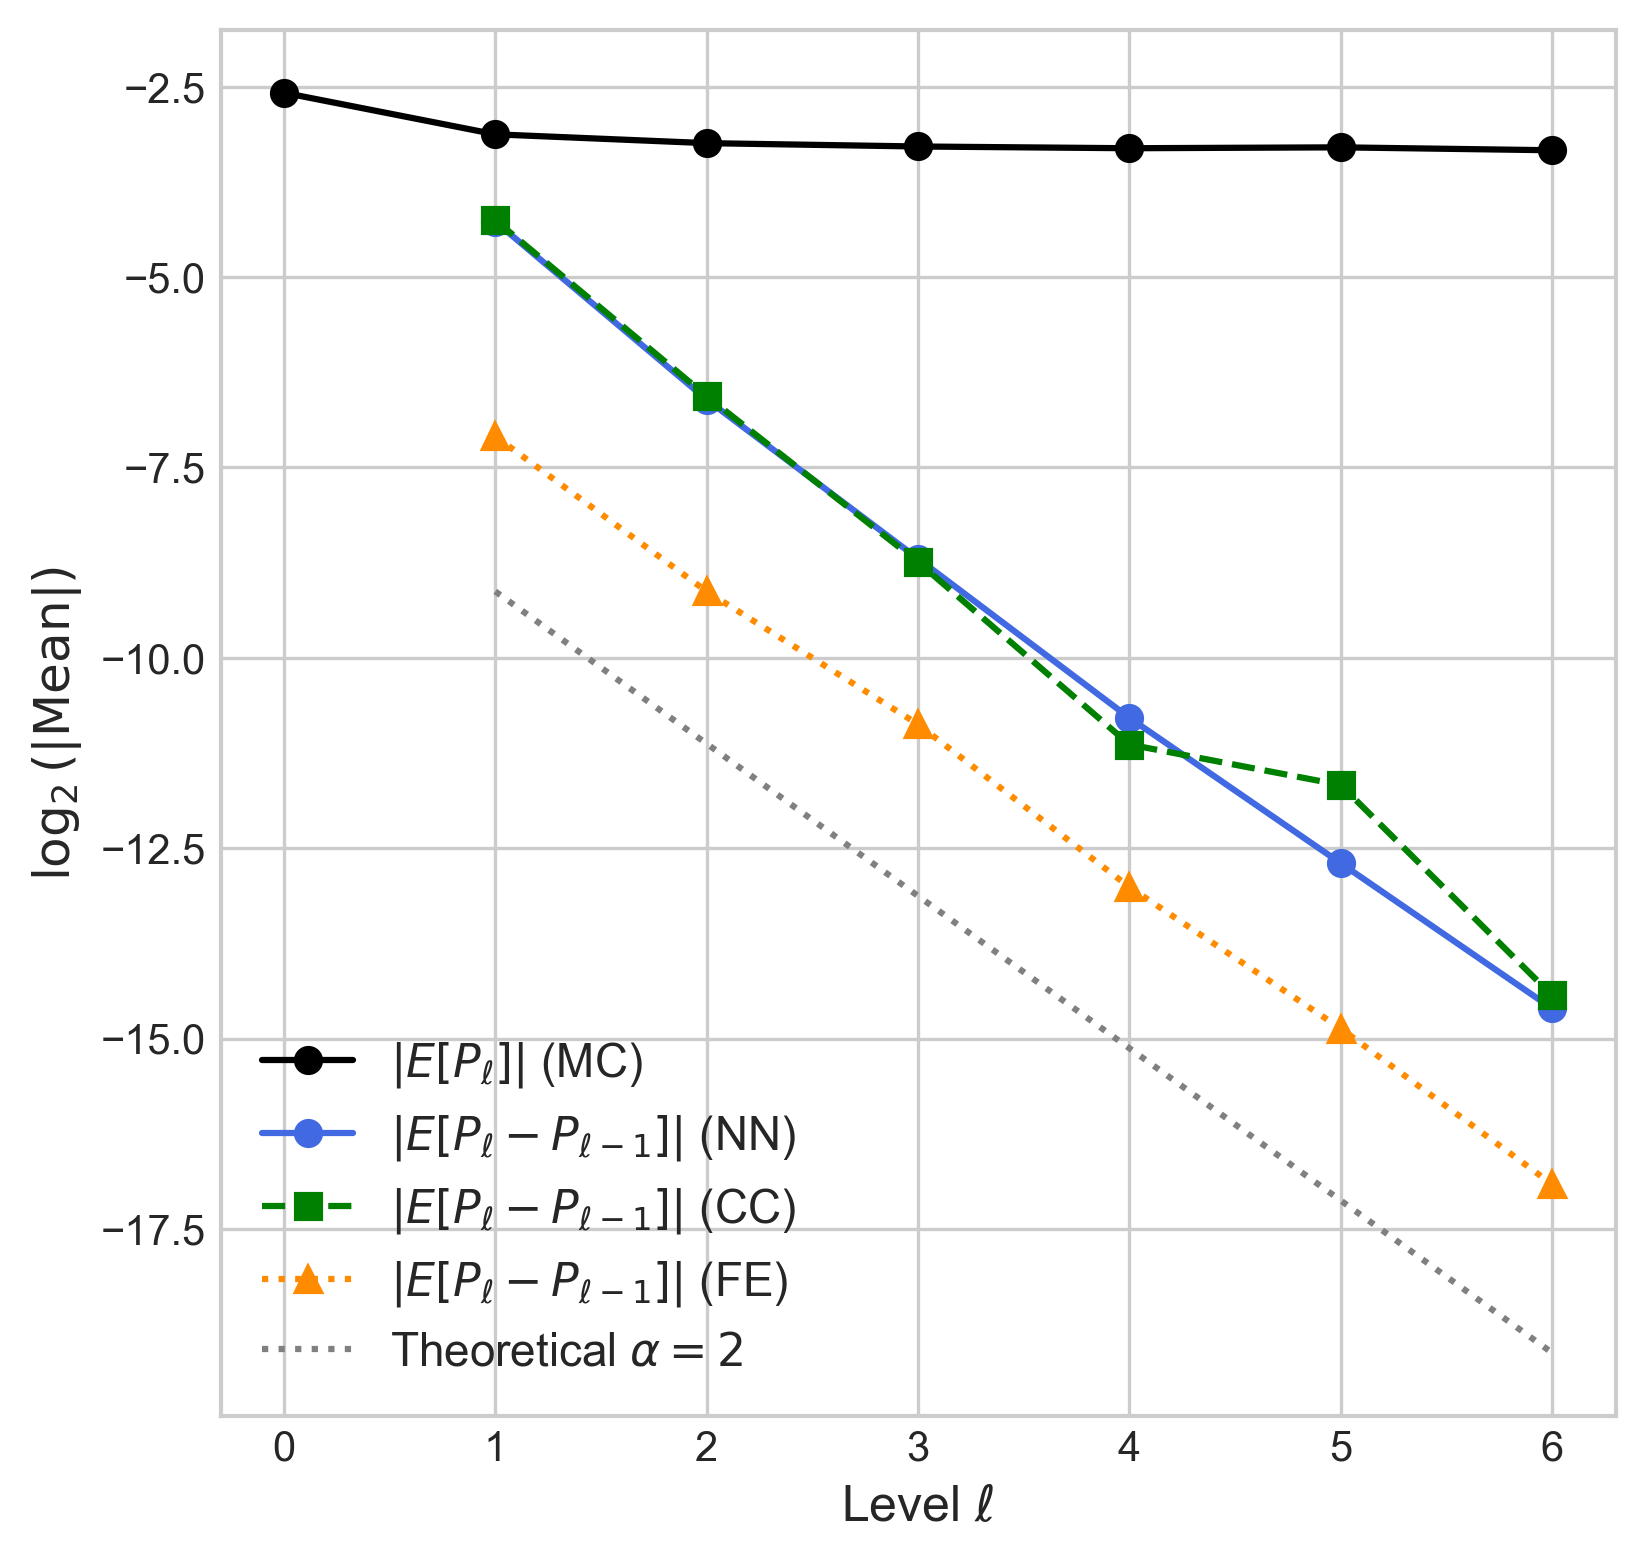
\includegraphics[width=\linewidth]{graphics/she_sq_amp_err_decay.png}
            \caption{Weak error convergence ($\alpha$).}
            \label{fig:she_sq_amp_mean_decay}
        \end{subfigure}
        \hfill
        \begin{subfigure}[b]{0.48\textwidth}
            \centering
            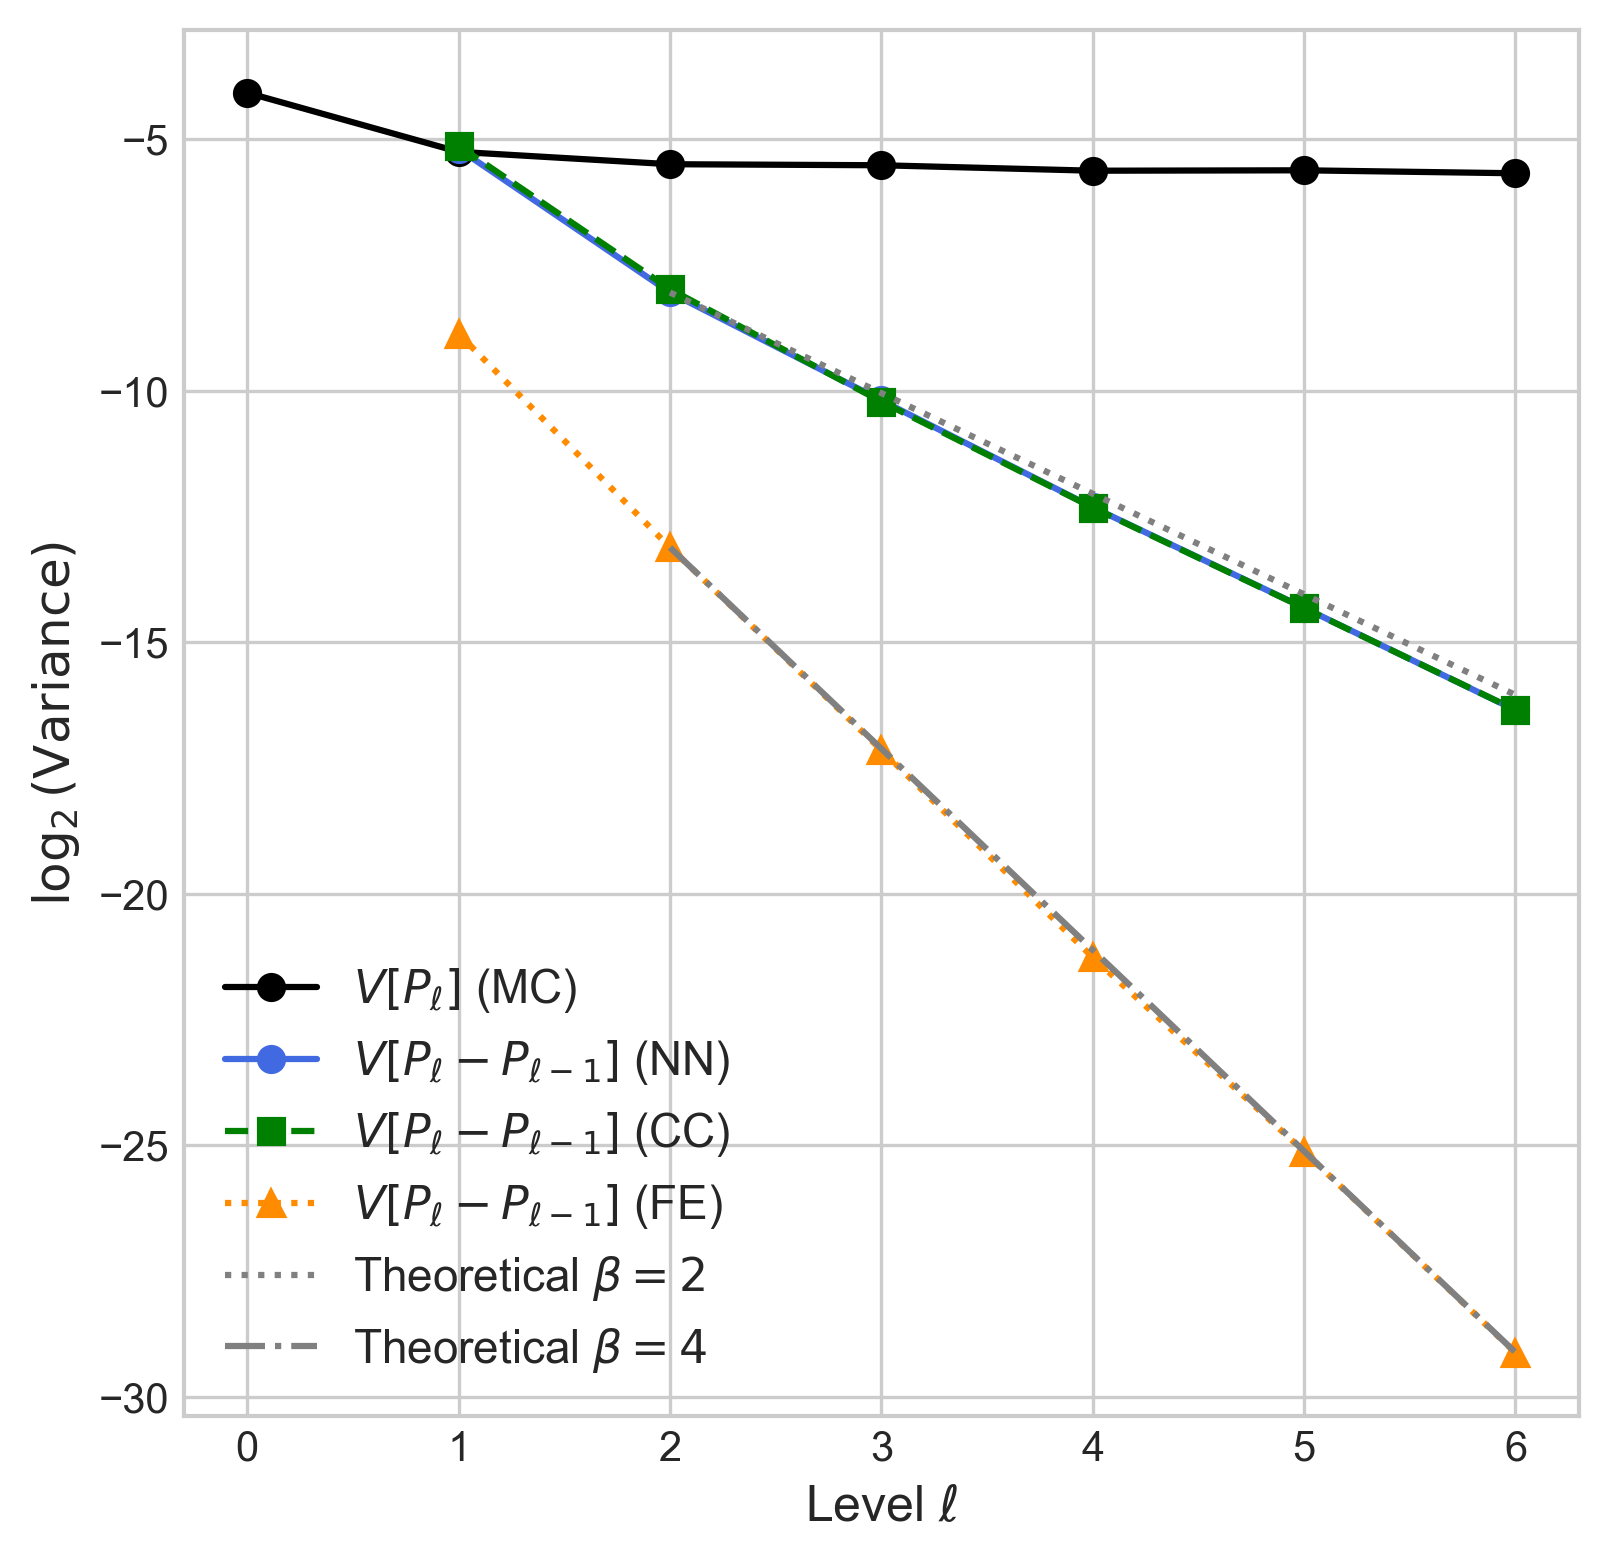
\includegraphics[width=\linewidth]{graphics/she_sq_amp_var_decay.png}
            \caption{MLMC variance decay ($\beta$).}
            \label{fig:she_sq_amp_variance_decay}
        \end{subfigure}        
    \end{subfigure}
    \vspace{1cm}
    \begin{subfigure}{\textwidth}
        \centering
        \begin{subfigure}[b]{\textwidth}
            \centering
            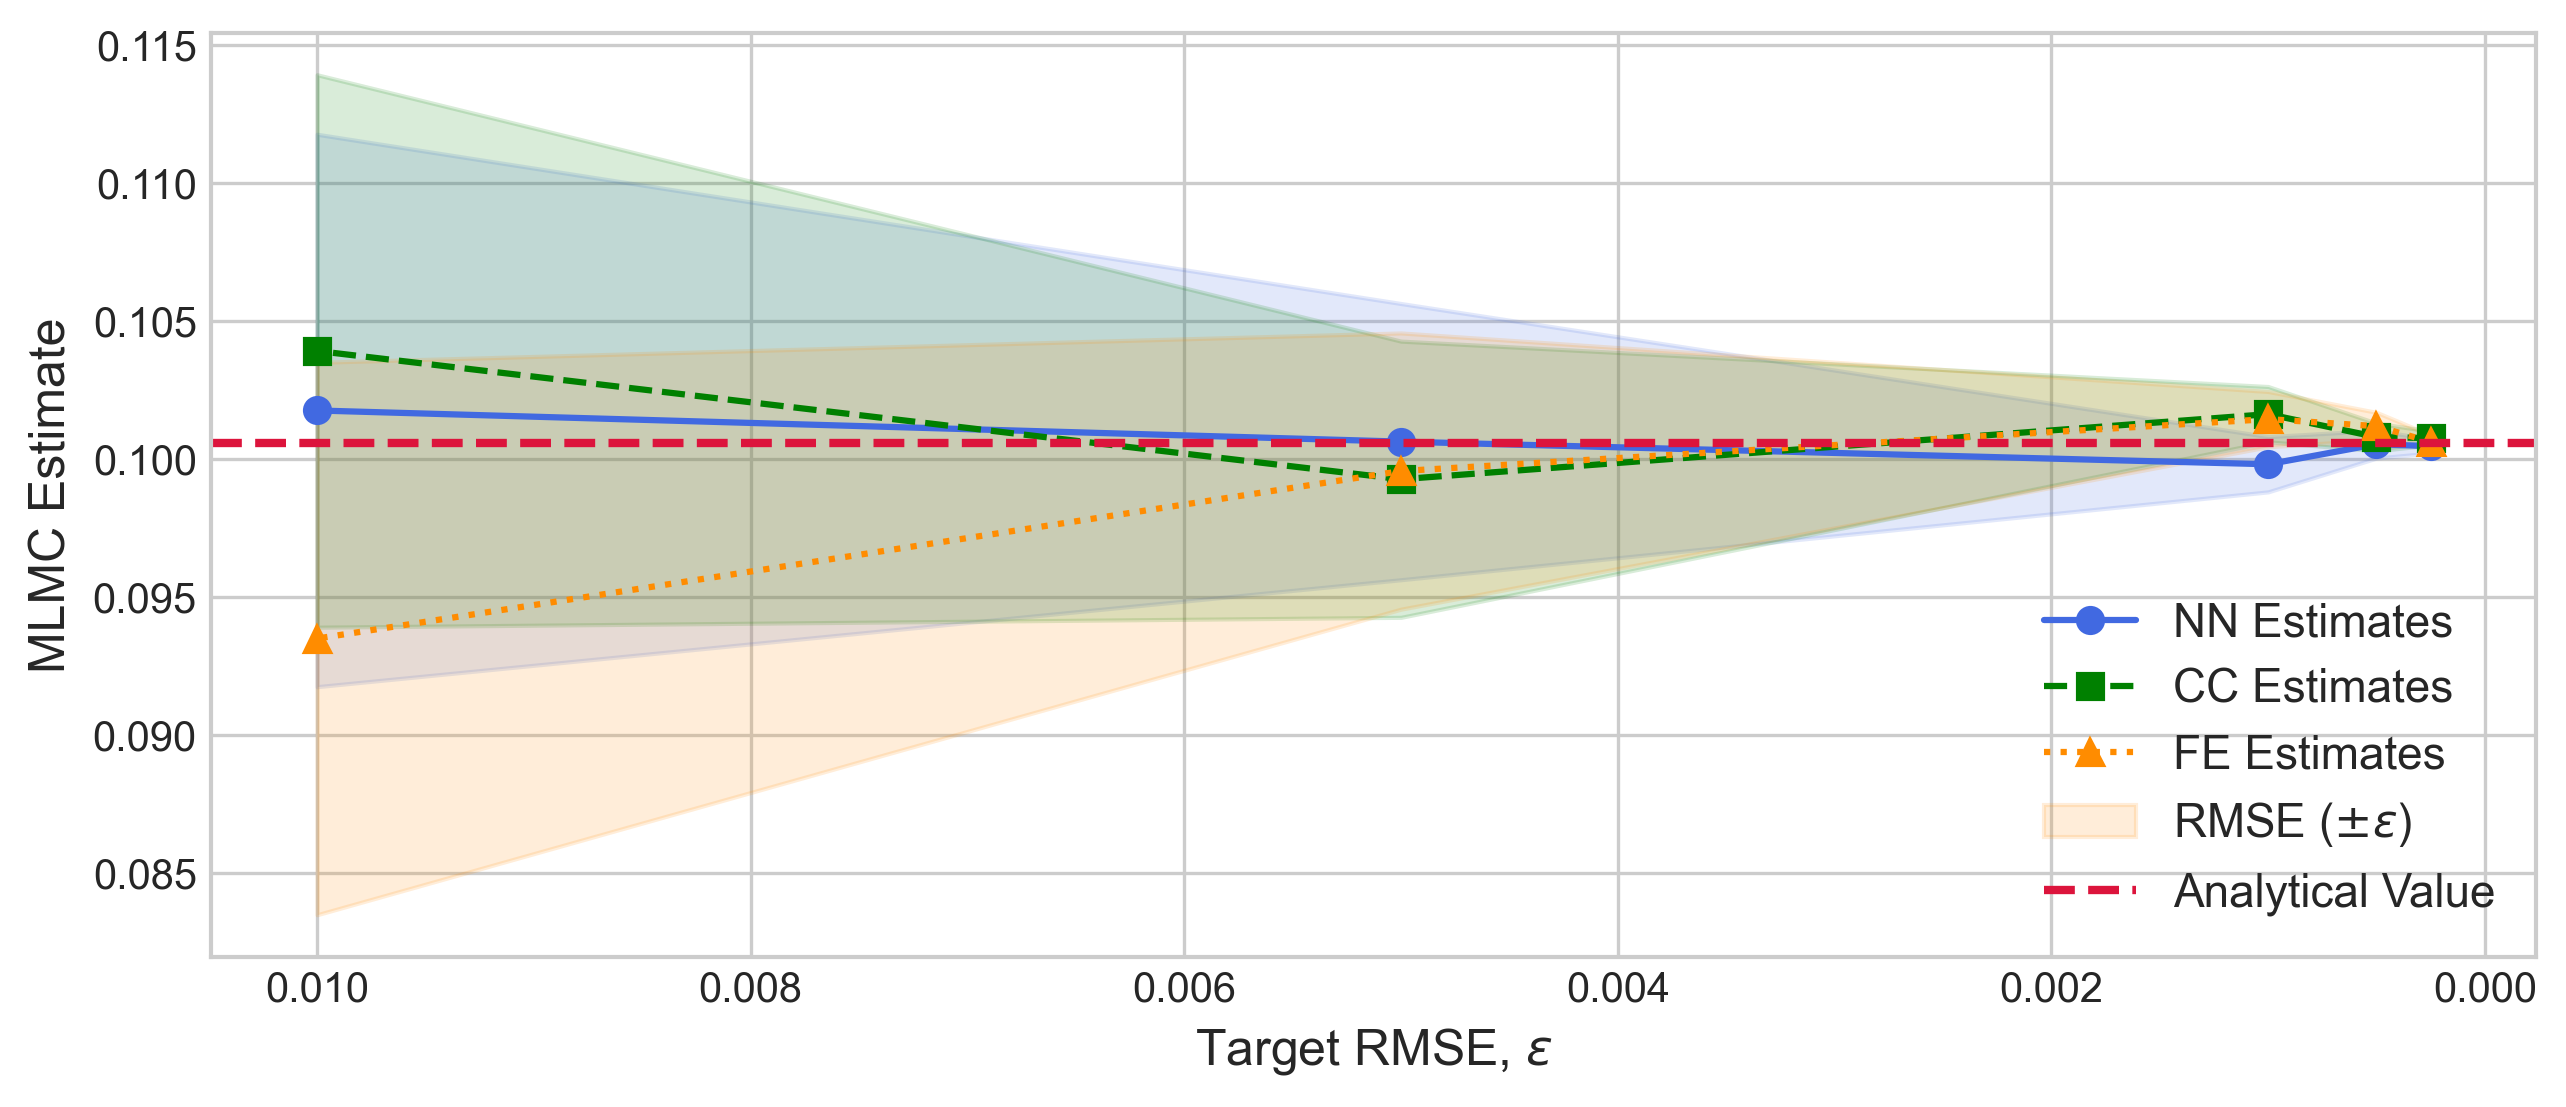
\includegraphics[width=0.7\linewidth]{graphics/she_sq_amp_conv.png}
            \caption{Final MLMC estimate vs. target RMSE ($\varepsilon$).}
            \label{fig:she_sq_amp_conv_vs_eps}
        \end{subfigure}
        \vspace{0.5cm}
        \begin{subfigure}[b]{\textwidth}
            \centering
            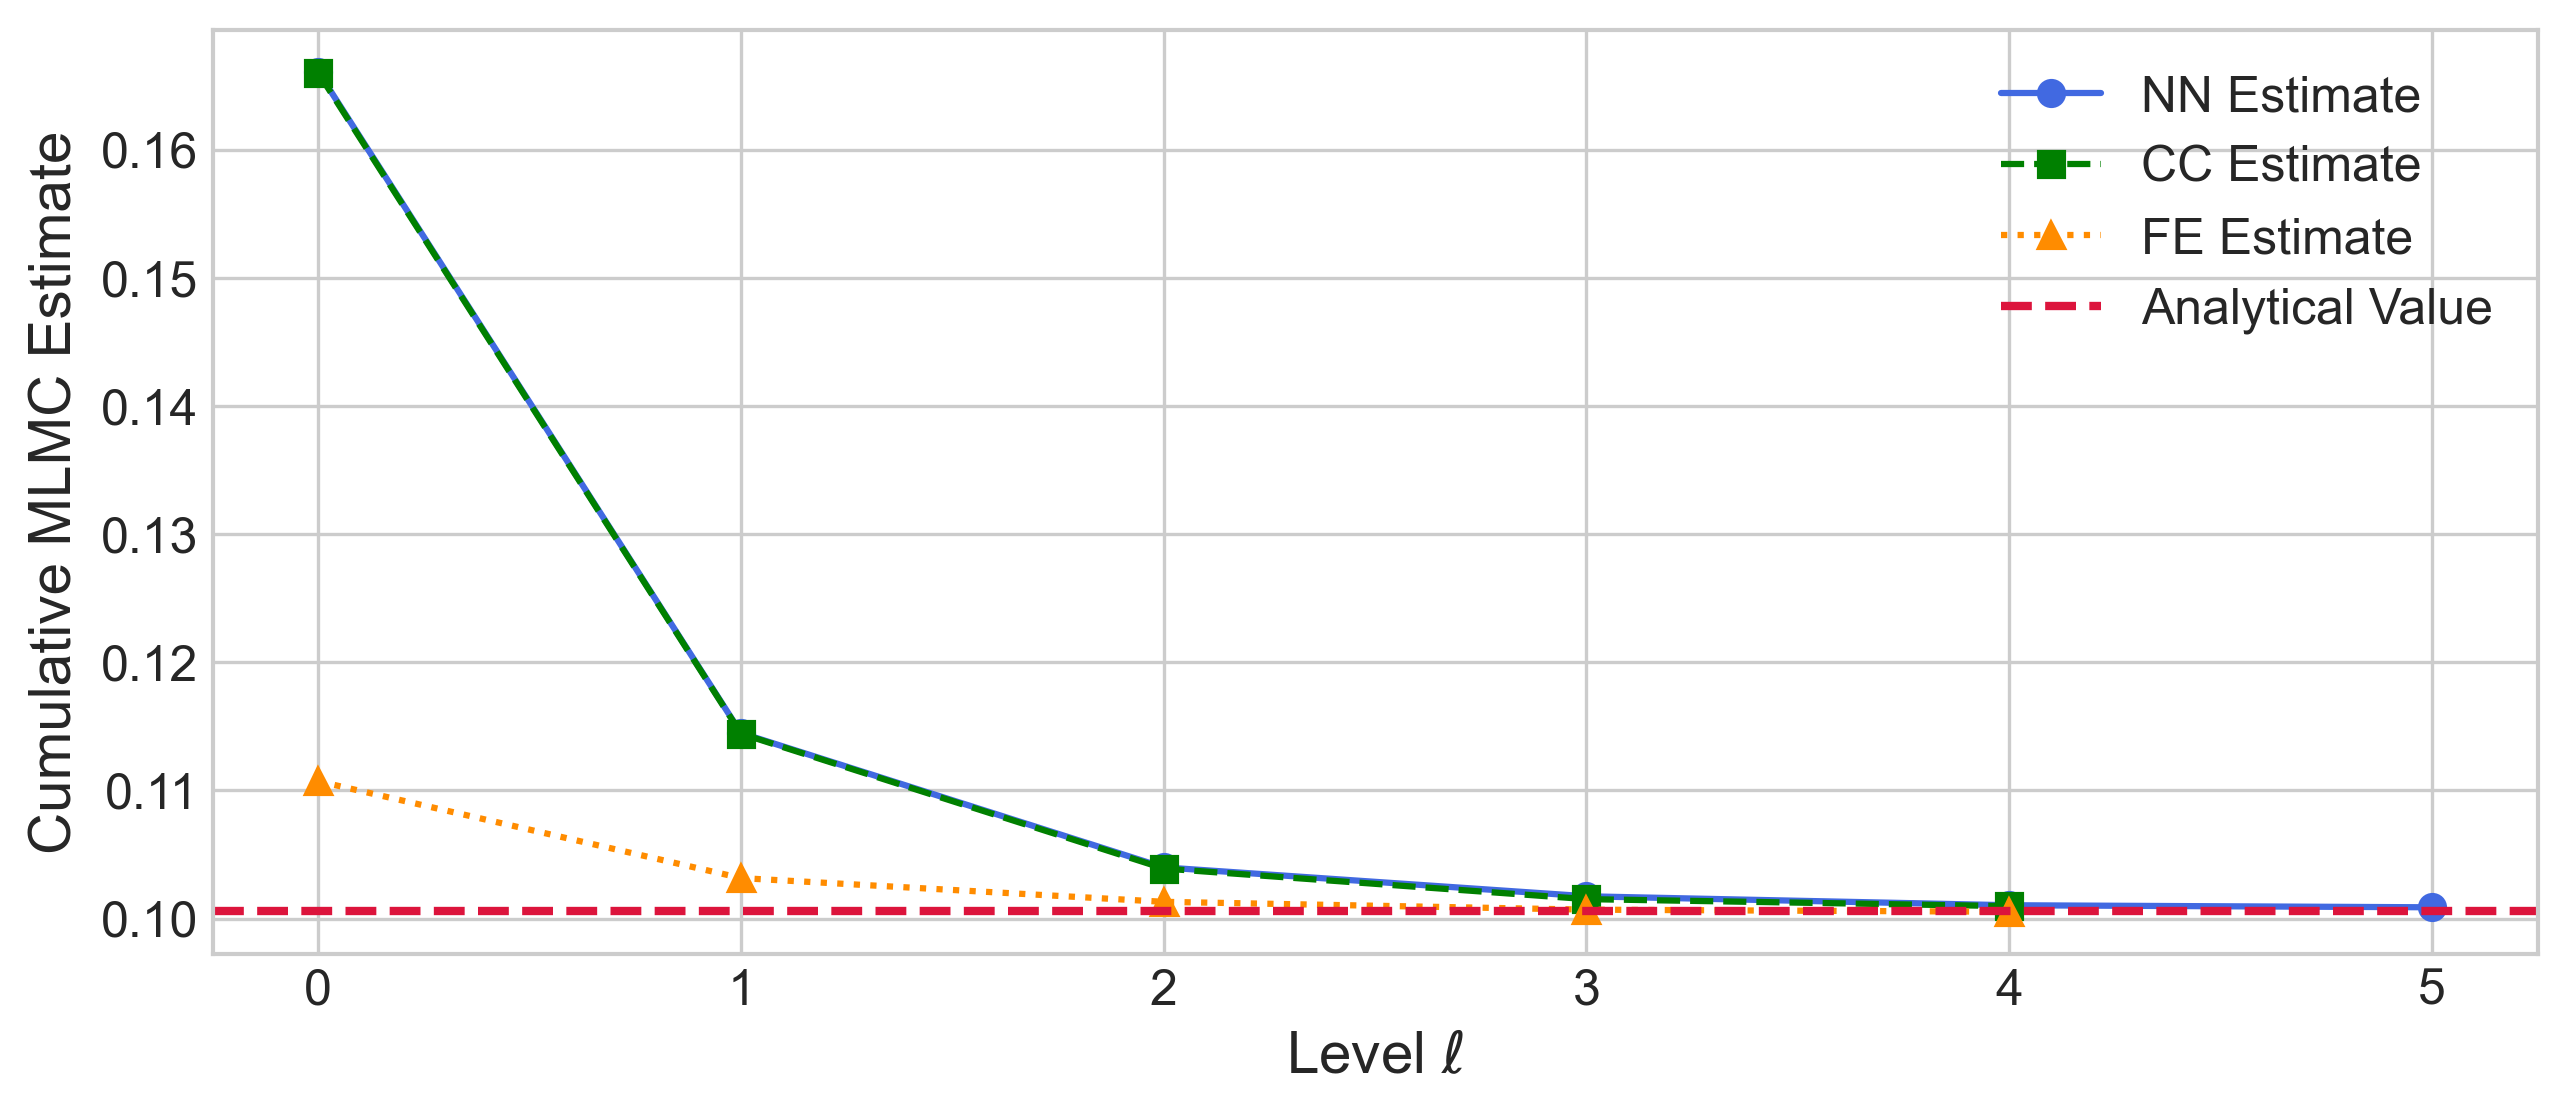
\includegraphics[width=0.7\linewidth]{graphics/she_sq_amp_cumconv.png}
            \caption{Cumulative estimate vs. level ($\ell$) for $\varepsilon=0.001$.}
            \label{fig:she_sq_amp_cumulative_conv}
        \end{subfigure}
    \end{subfigure}
    \caption{Decay and convergence plots for the MLMC implementation of the SHE, using the squared 
    amplitude of the first Fourier mode as our QoI.}
    \label{fig:she_validation_combined}
\end{figure}


We first comment on the rates observed. In line with our expectations for a one-dimensional 
problem, 
we observe $\gamma = 3$ across 
all couplings. Similarly, we obtain estimates of $\alpha \approx 2$ for all coupling methods,
consistent with Proposition \ref{prop:weak_error_for_fourier_mode} which 
established that the weak convergence rate was independent of coupling.
Figure \ref{fig:she_sq_amp_mean_decay} illustrates this behaviour. Notably,
while the NN and CC couplings exhibit almost identical magnitudes of weak error across 
levels, the FE method consistently yields a smaller 
weak error across levels, the FE method displays a smaller weak error.

The most critical distinction between the couplings arises in the variance decay, 
shown in Figure \ref{fig:she_sq_amp_variance_decay}. Here, the FE method 
achieves the optimal decay rate of $\beta = 4$. Following Proposition 
\ref{prop:variance_decay_fourier}, this behaviour infers that the FE method 
achieves perfect correlation, between the coarse and fine samples at each level. 
By contrast, the CC method,
although more correlated than the NN method, does not 
achieve perfect correlation as indicated by its alignment with the 
variance decay of the NN method. As expected, the NN method 
has $\beta = 2$, since it discards a portion of the fine-grid randomness when 
constructing coarse increments.

For comparison, we also include the behaviour of the standard Monte Carlo 
estimator. Using 10,000 samples at each level, we observe no error decay 
or variance reduction, as expected.

The most critical distinction between the methods is revealed in the variance decay,
shown in Figure \ref{fig:she_sq_amp_variance_decay}. We observe that the FE method
achieves the optimal decay rate of $\beta = 4$, 
We can infer, following 
Proposition \ref{prop:variance_decay_fourier}, that FE coupling achieves 
perfect correlation between levels while the CC method does not. We knew the 
NN method would not, as it discards some noise.

We also include the MC estimator's means and variances, obtained also using $10,000$ samples
at each level reported. We observe no error or variance decay in the MC estimator, which 
also aligns with our expectations.

Finally, Figures \ref{fig:she_sq_amp_conv_vs_eps} and \ref{fig:she_sq_amp_cumulative_conv}
demonstrate convergence of the MLMC implementation for all coupling methods.
In Figure \ref{fig:she_sq_amp_cumulative_conv}, we observe that 
the convergence speeds differ, though, with the FE method converging significantly
faster than the NN and CC methods. We observe that the FE and CC methods only requires progressing 
to the fourth level, while the NN method progresses to the fifth. This is attributable 
to the intrinsic stochasticity of the system affecting the stopping criterion 
of the MLMC Algorithm, outlined in Algorithm \ref{alg:mlmc_detailed}.

We now provide similar validation results for our SHE MLMC implementation, where our QoI is the system energy. 
We have the true value for the problem, $\approx \frac{1}{12}$, via
\ref{eq:she_energy_analytic_soln}.

\begin{table}[htbp]
    \centering
    \begin{tabular}{|l|c|c|r|}
        \hline
        \textbf{Coupling Method} & \textbf{$\alpha$} & \textbf{$\beta$} & \textbf{$\gamma$} \\
        \hline
        Nearest Neighbour & 0.58 & 2.14 & 3.02\\
        Central Coupling & 0.54 & 2.17 & 3.03 \\
        Finite Element & 1.16 & 2.96 & 3.0 \\
        \hline
    \end{tabular}
    \caption{Empirically estimated rates for the system energy}
    \label{tab:energy_decay_rates}
\end{table}

\begin{figure}[htbp]
    \centering
    \begin{subfigure}{\textwidth}
        \centering
        \begin{subfigure}[b]{0.48\textwidth}
            \centering
            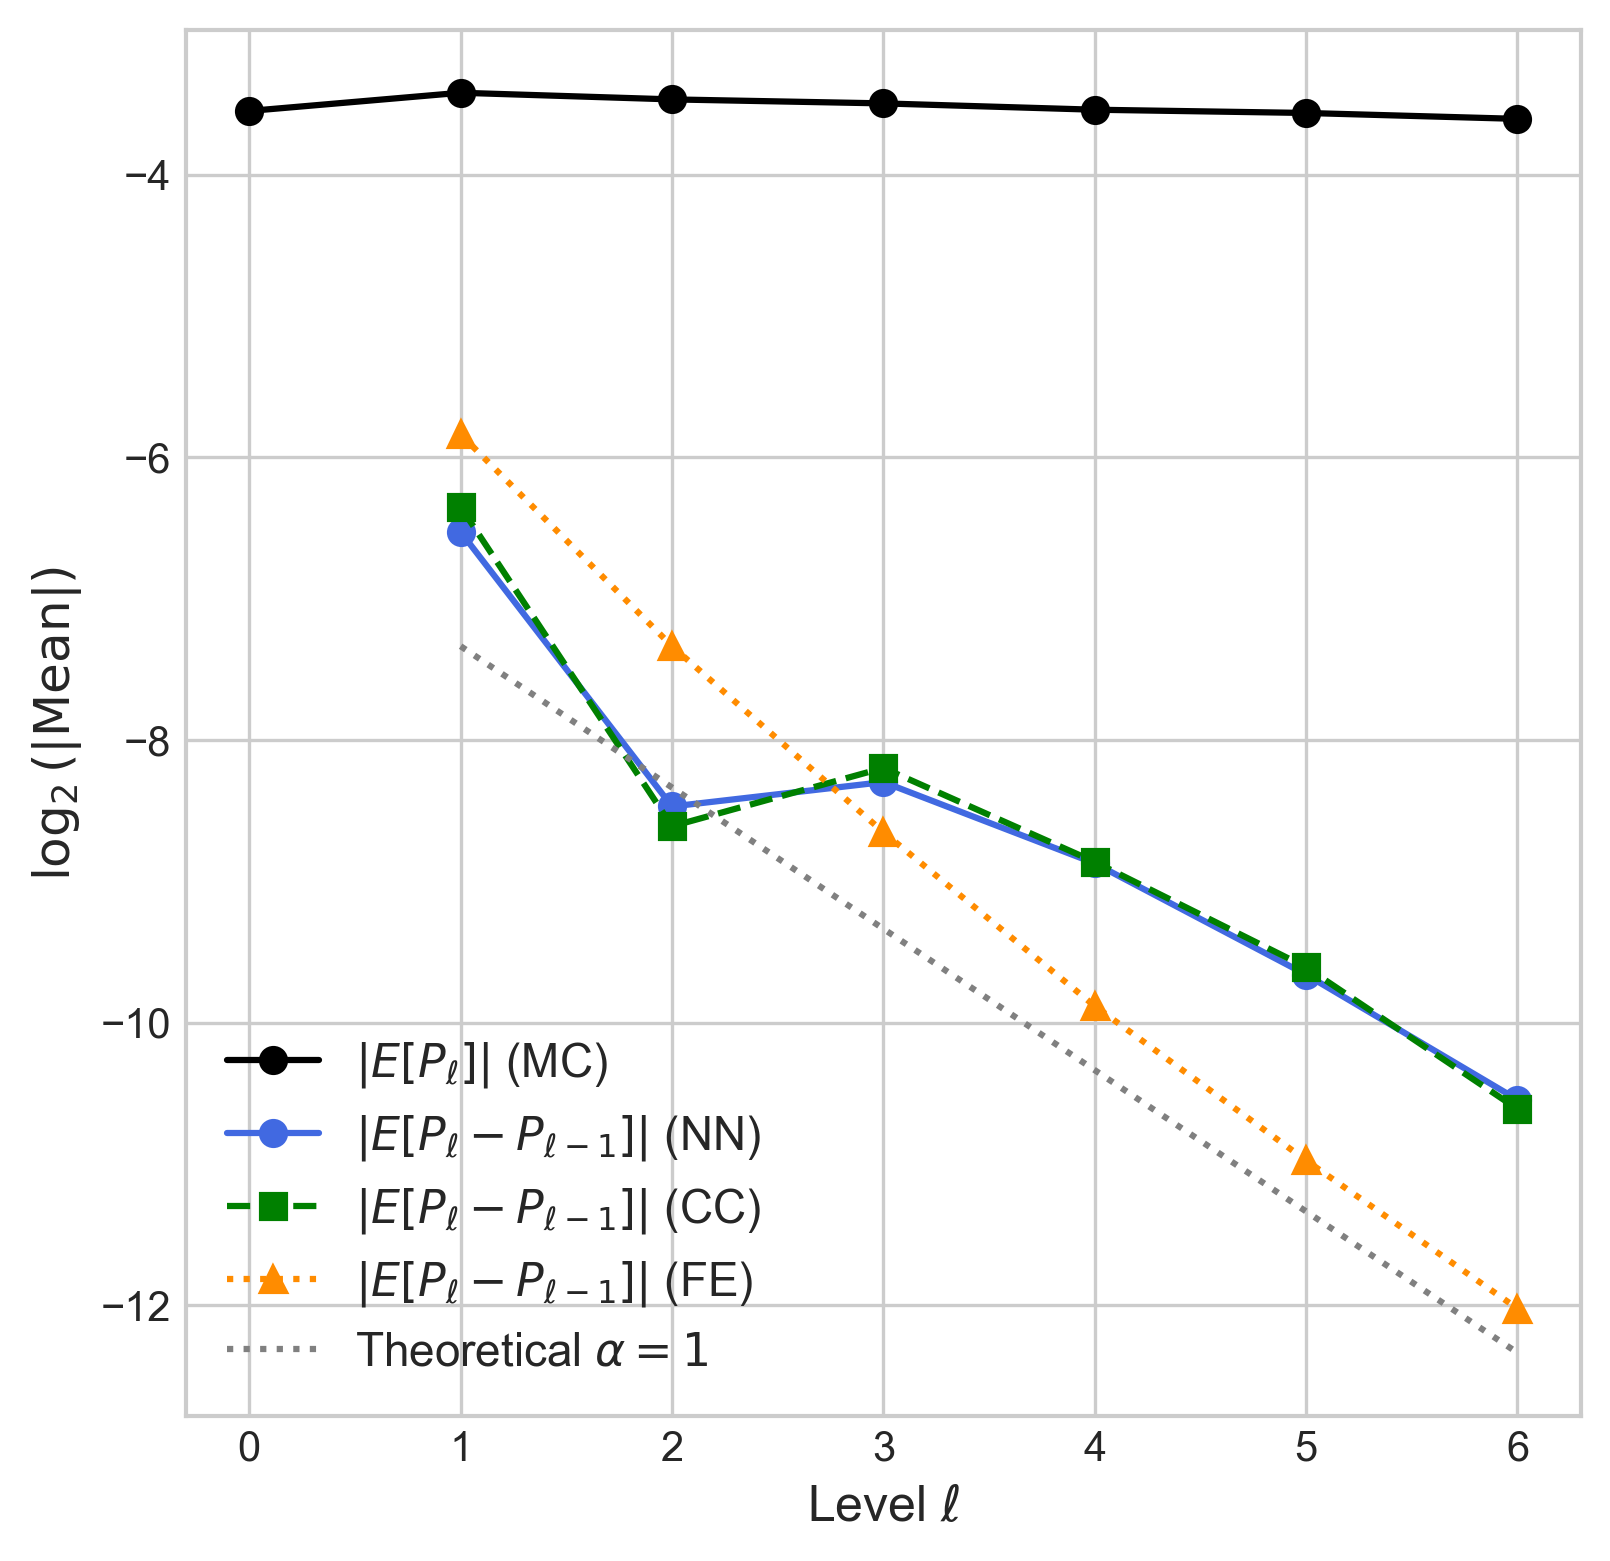
\includegraphics[width=\linewidth]{graphics/she_energy_err_decay.png}
            \caption{Weak error convergence ($\alpha$).}
            \label{fig:energy_mean_decay}
        \end{subfigure}
        \hfill
        \begin{subfigure}[b]{0.48\textwidth}
            \centering
            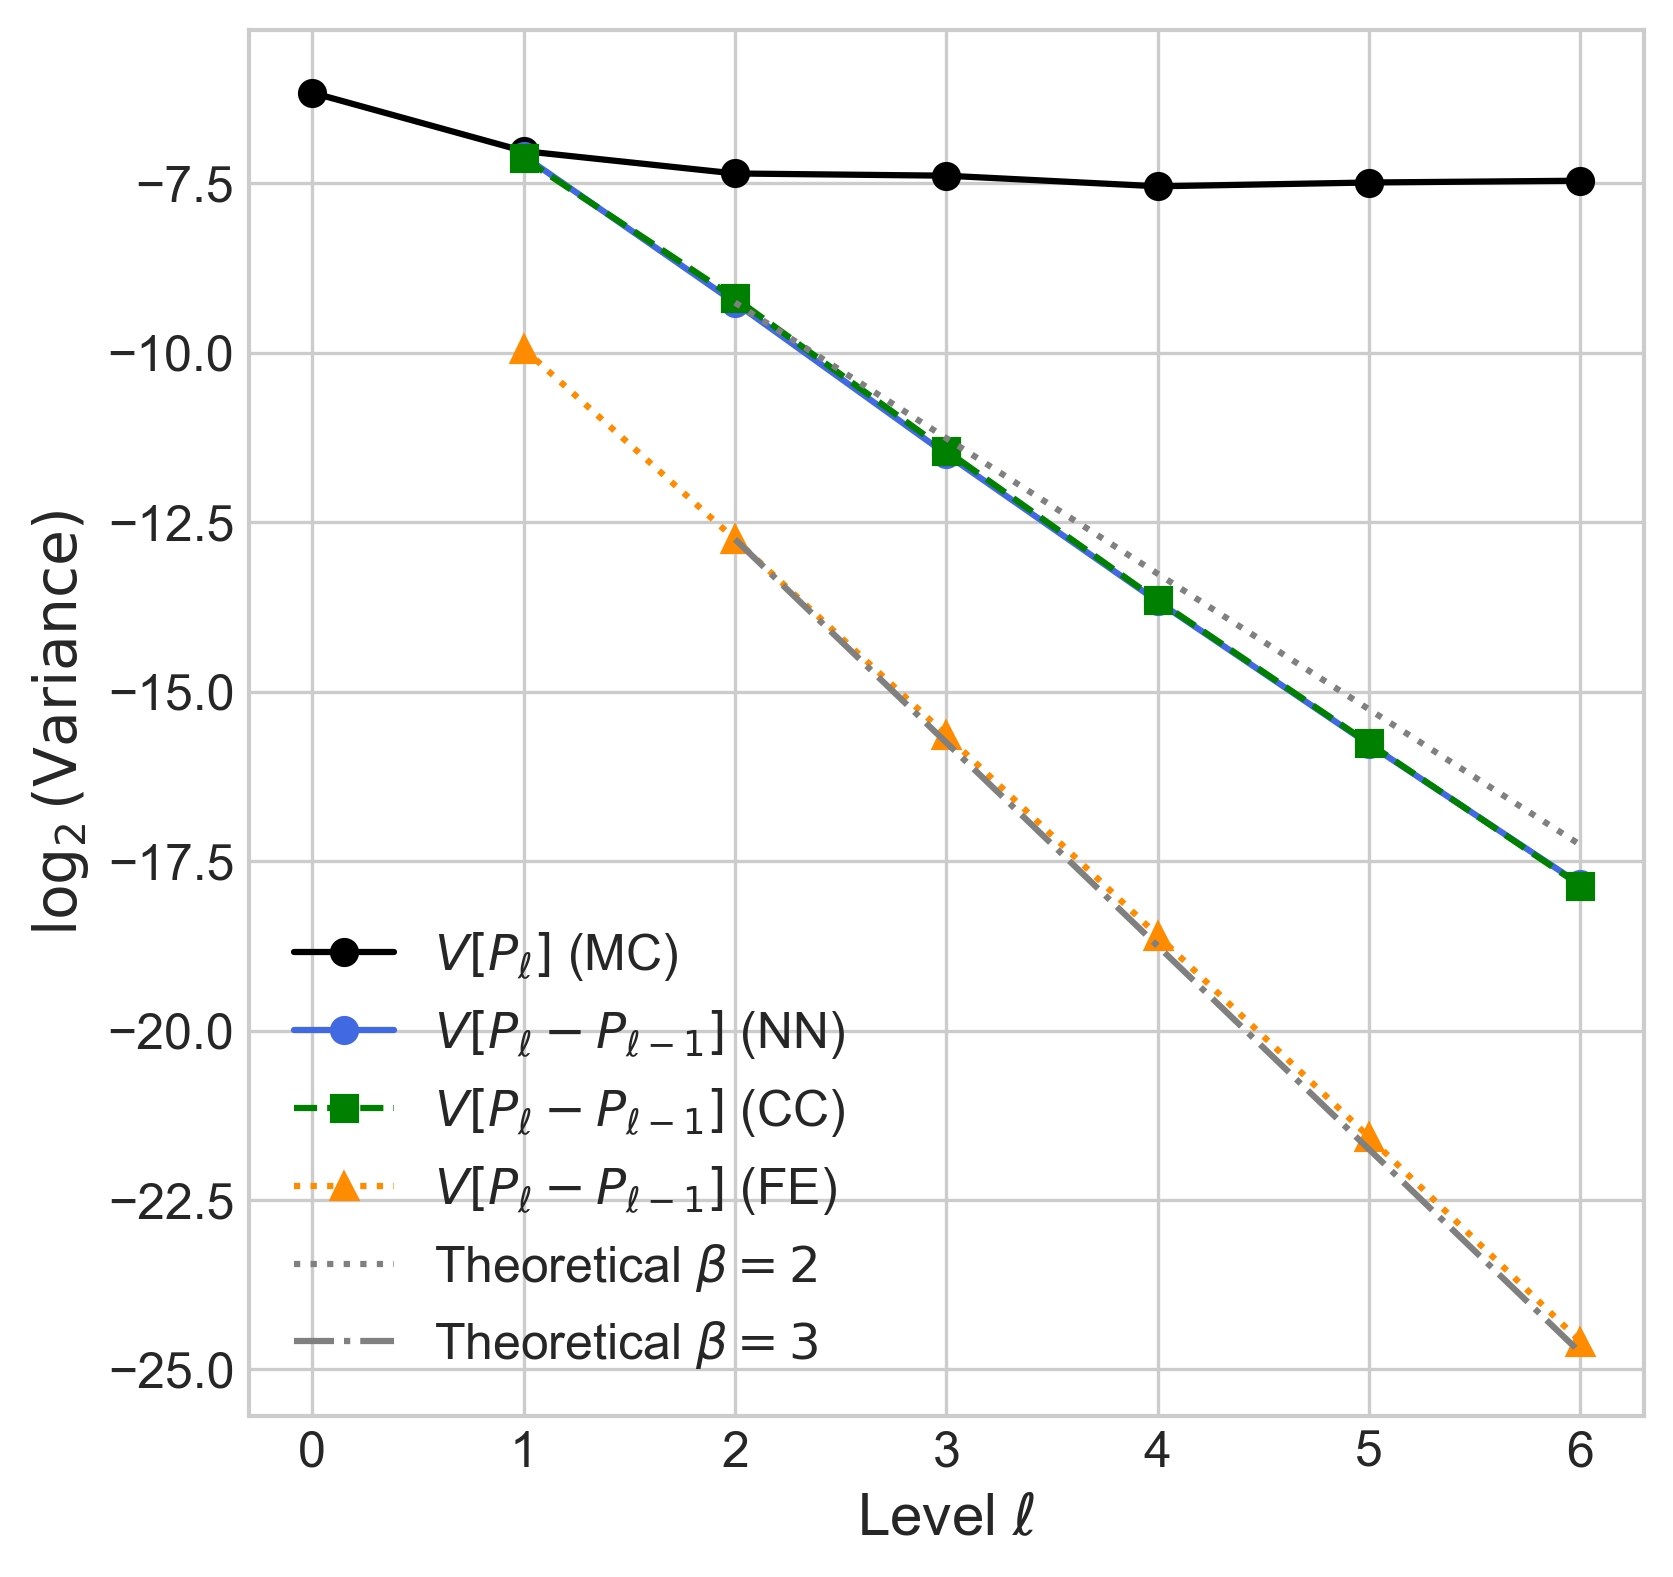
\includegraphics[width=\linewidth]{graphics/she_energy_var_decay.png}
            \caption{MLMC variance decay ($\beta$).}
            \label{fig:energy_variance_decay}
        \end{subfigure}
    \end{subfigure}
    \vspace{1cm}
    \begin{subfigure}{\textwidth}
        \centering
        \begin{subfigure}[b]{\textwidth}
            \centering
            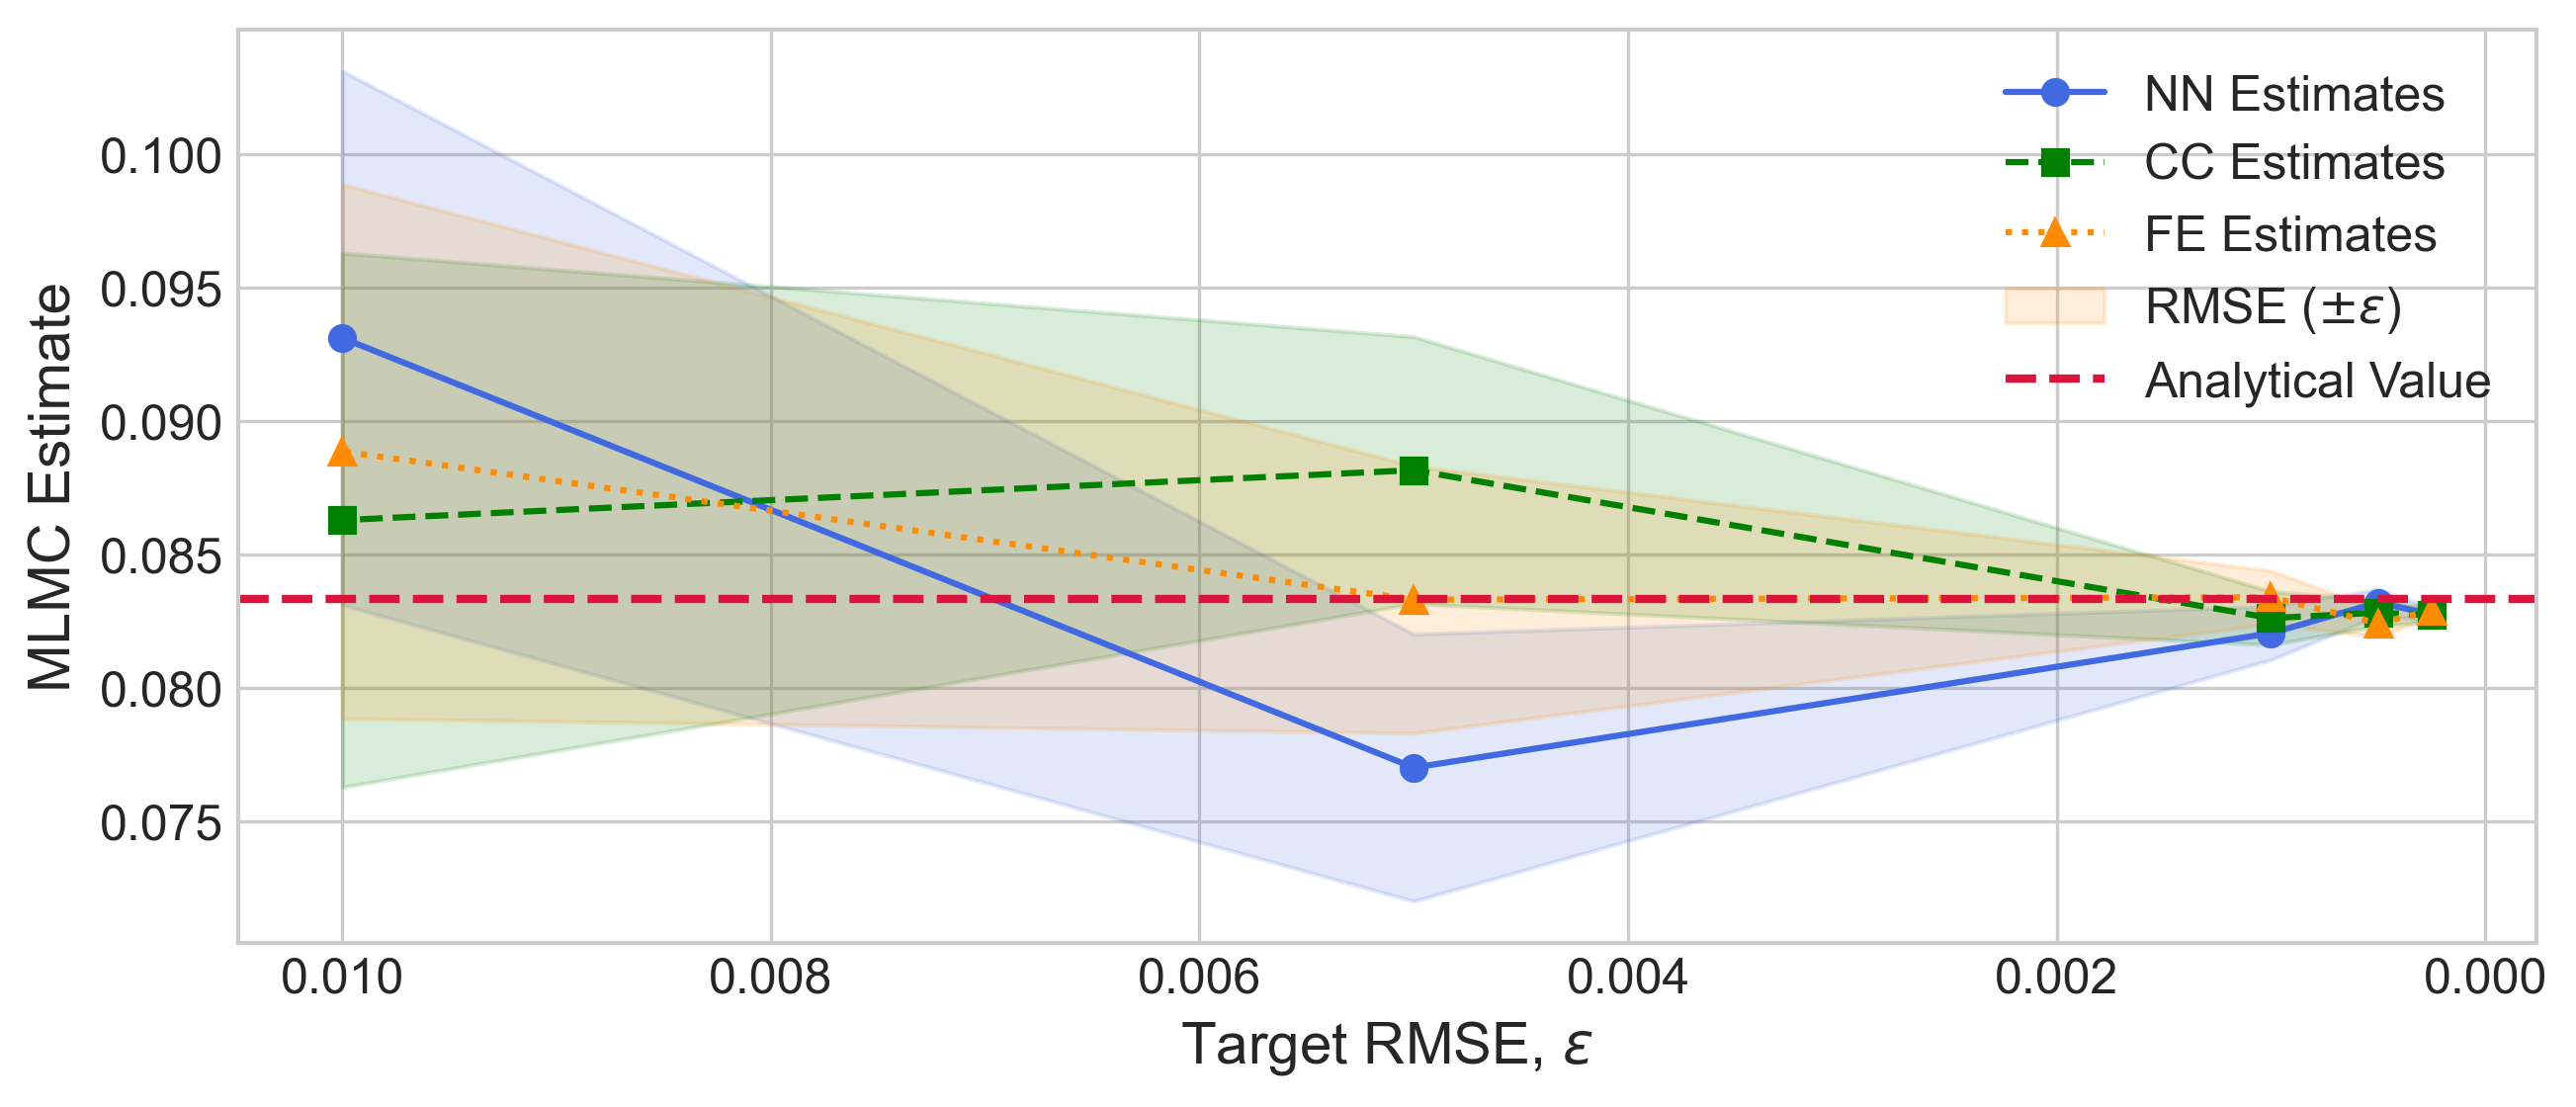
\includegraphics[width=0.7\linewidth]{graphics/she_energy_conv.png}
            \caption{Final MLMC estimate vs. target RMSE ($\varepsilon$).}
            \label{fig:energy_conv_vs_eps}
        \end{subfigure}
        \vspace{0.5cm}
        \begin{subfigure}[b]{\textwidth}
            \centering
            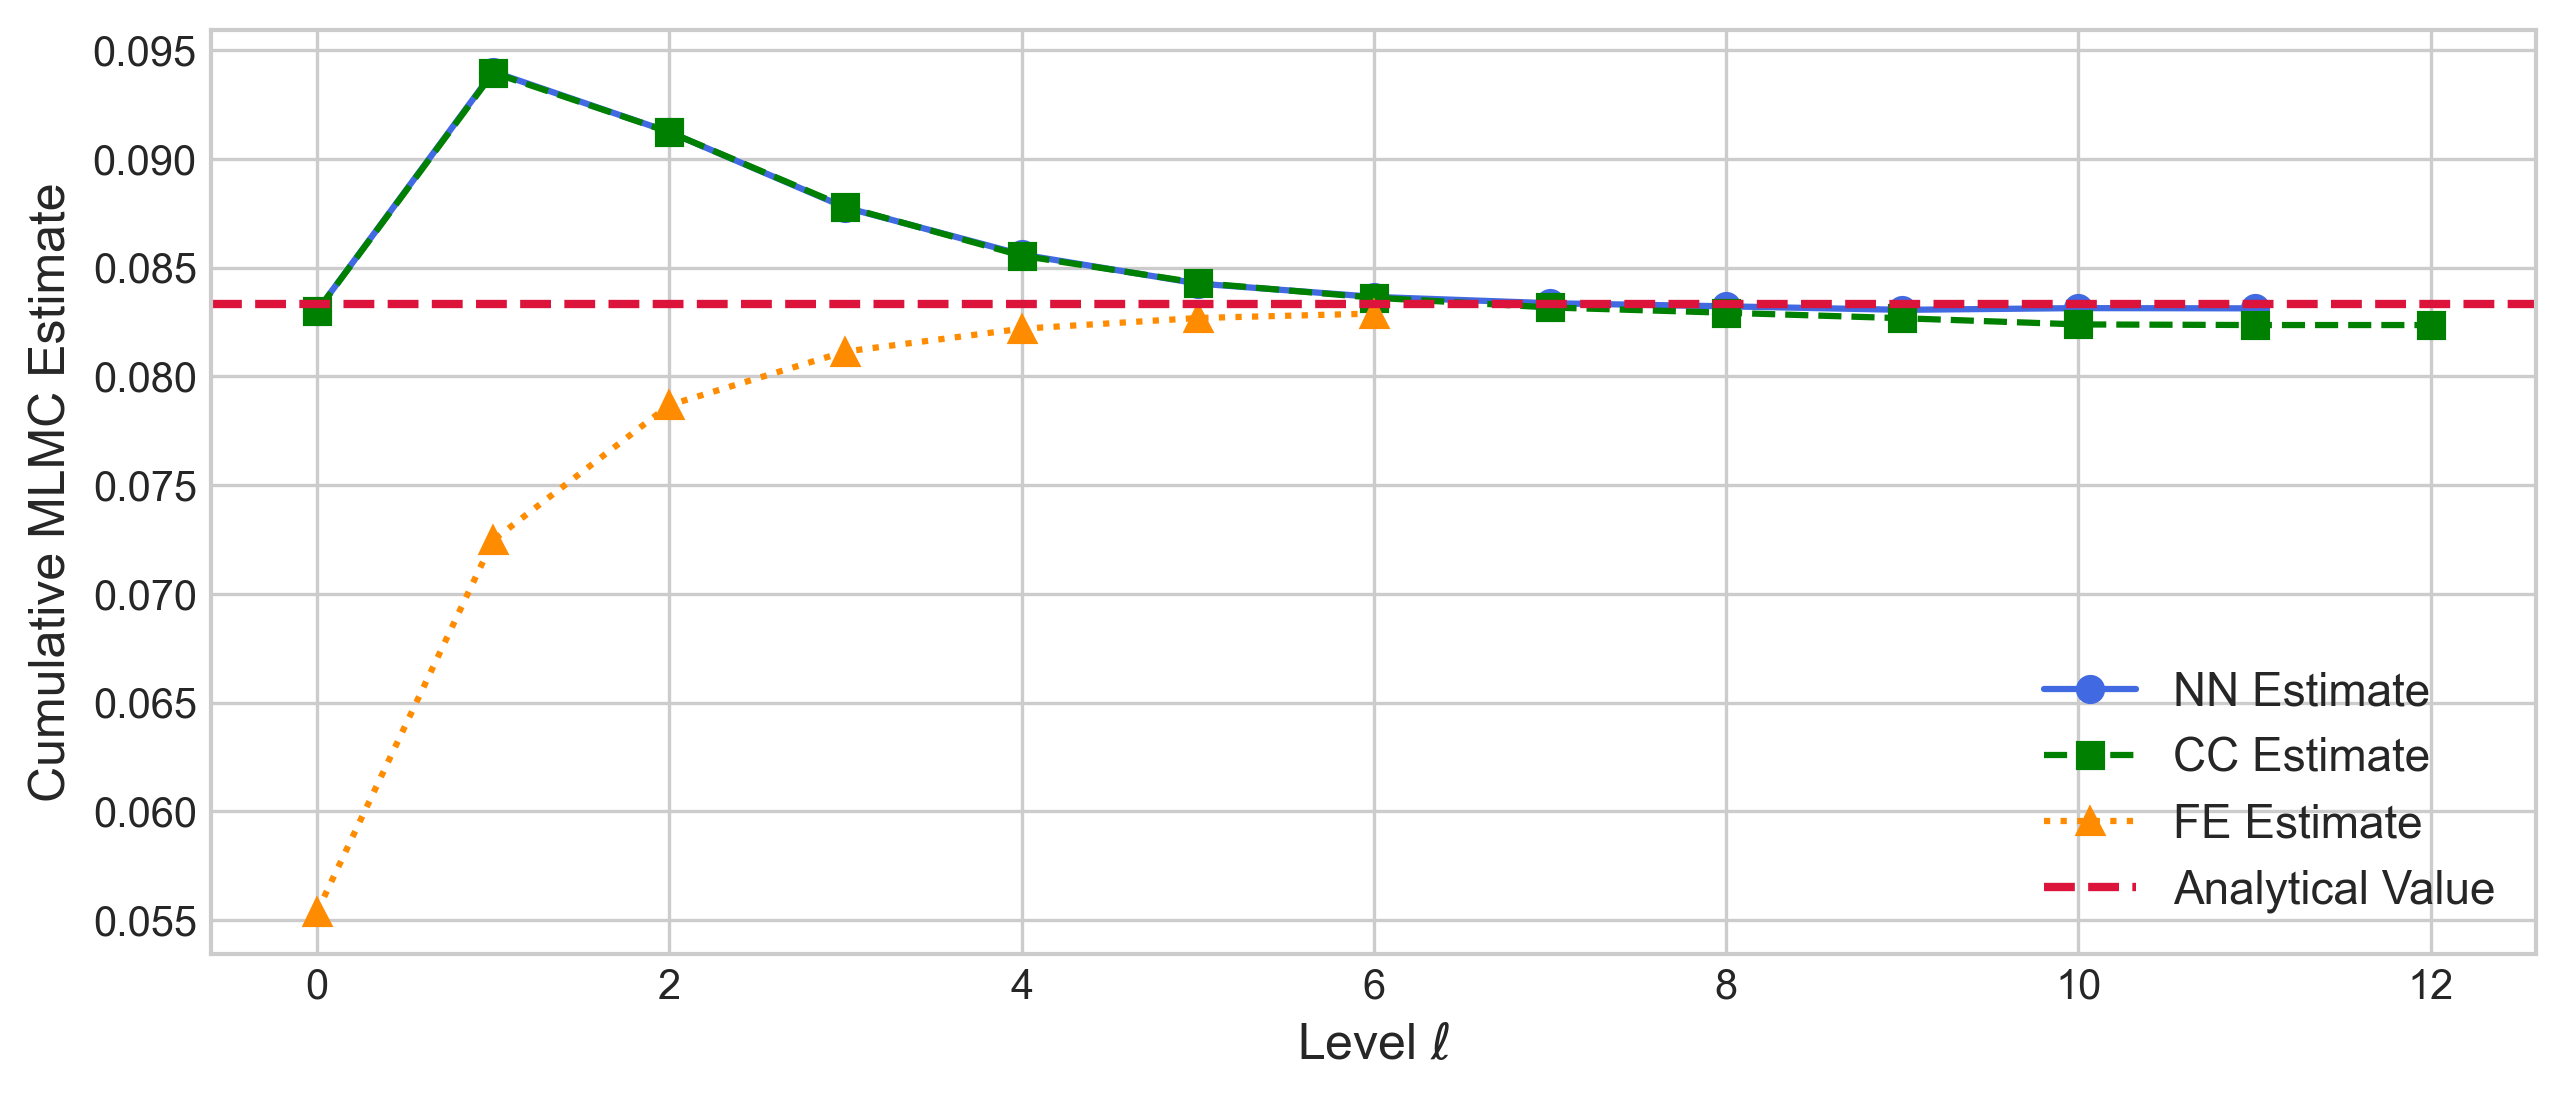
\includegraphics[width=0.7\linewidth]{graphics/she_energy_cumconv.png}
            \caption{Cumulative estimate vs. level ($\ell$) for $\varepsilon=0.001$.}
            \label{fig:energy_cumulative_conv}
        \end{subfigure}
    \end{subfigure}
    \caption{Decay and convergence plots for the MLMC implementation of the SHE,
    using the system energy as our QoI.}
    \label{fig:she_validation_combined}
\end{figure}


The rates shown in Table \ref{tab:energy_decay_rates} and Figures 
\ref{fig:energy_mean_decay} and \ref{fig:energy_variance_decay} 
are quite different to those obtained for the squared amplitude. 
We observe $\gamma = 3$, as expected for this system. However, 
for the energy we have a slower error decay. $\alpha \approx 1$ for the 
FE method, $\alpha \approx 0.5$ for the NN and CC methods. Examining 
Figure \ref{fig:energy_mean_decay}, which shows the samples used to estimate 
$\alpha$ for the three mechanisms, we see the source of the discrepancy is 
due to a kink in the NN and CC weak errors observed, occurring at $\ell = 2$. 
Otherwise, the expected decay rate would have been 1 for all coupling mechanisms.
This difference from the squared amplitudes is interesting.

Similarly, for the variance decay, we observe again that the FE method
achieves improved variance decay compared to the NN and CC methods, but 
not to the same extent, achieving $\beta \approx 3$ compared to 
$\beta \approx 2$. As we know that the 
FE coupling perfectly correlates samples at adjacent levels, we 
can infer that $\beta = 3$ is the largest decay rate achievable.

Convergence to the true value is observed across all methods 
and all RMSE targets. In Figure \ref{fig:energy_conv_vs_eps}, 
we see a clear trend towards the analytic 
solution as accuracy increases (i.e., RMSE decreases). A key 
distinction arises in 
the cumulative convergence behaviour, shown in Figure 
\ref{fig:energy_cumulative_conv}. Here, significantly more levels 
are required to achieve the desired RMSE compared to the squared
amplitude case. The FE method converges at approximately 
level 7, while both NN and CC require progression to levels 
12 and 11. This is a direct consequence of slower 
weak error decay (equivalently, larger $\alpha$). 
The larger value means that more levels are required to 
sufficiently reduce the discretisation error.

We also observe that the NN and CC estimates are functionally identical
at small RMSEs, Figure \ref{fig:energy_cumulative_conv}. Their values 
do differ slightly, but the differences 
are negligible. This is not observed for lower RMSEs.

% Finally, we comment on the observation that in Figure \ref{fig:energy_cumulative_conv}, 
% for both the NN and CC methods the cumulative estimates move away before 
% gradually converging back. We attribute this behaviour to 
% the first level estimator having large variance 
% compared to the initial level $\ell = 0$ estimate.
